\documentclass[french,a4paper,10pt]{article}
% uncomment the following lines after copying the template
\input{../../common/common_header.tex}
\input{../../common/macros/math.tex}
\input{../../common/macros/theorems.tex}
% ============================================================================== 
% GENERAL MATH SHORTCUTS
% ==============================================================================

\newcommand{\abs}[1]{\left\lvert#1\right\rvert}  % Absolute value with scalable bars
\counterwithout{tdcounter}{section} 
\usetikzlibrary{shapes,arrows,positioning,calc,fit,backgrounds,angles,quotes}
% \newcommand{\becomes}{\begin{center}\(\downarrow\)\end{center}}


% ============================================================================== 
% JULIA CODE STUFF
% ==============================================================================


\usepackage{floatrow}
\usepackage{caption}
\usepackage{cases}


\usepackage{listings}
\usepackage{xcolor}

% ----- Julia language definition -----
\lstdefinelanguage{julia}{
    keywords={function, end, if, else, elseif, while, for, in, return, break, continue, struct, 
    mutable, using, import, module, export, const, let, global, local, abstract, typealias, 
    sin, atan, true, add},
    sensitive=true,
    comment=[l]{\#},
    morestring=[b]", % chktex 18
}
\definecolor{codebg}{RGB}{245,245,245}   % very light gray
\definecolor{codeborder}{RGB}{220,220,220} 
\definecolor{keywordcolor}{RGB}{0,0,150}
\definecolor{commentcolor}{RGB}{120,120,120}
\lstdefinestyle{julia-style}{
    language=julia, % new language
    basicstyle=\ttfamily\small,
    keywordstyle=\color{keywordcolor},
    commentstyle=\color{commentcolor},
    stringstyle=\color{verdant},
    backgroundcolor=\color{codebg},
    frame=single,
    framerule=0.5pt,
    rulecolor=\color{codeborder},
    tabsize=2,
    columns=fullflexible,
    keepspaces=true,
    showstringspaces=false,
}
% convenience macro
\newcommand{\juliaFile}[1]{\lstinputlisting[style=julia-style]{#1}}

% custom bash environment with same style as julia
\lstdefinelanguage{bash}{
    keywords={sudo, apt-get, install, update, upgrade, cd, ls, mkdir, rm, rmdir, touch, nano, vim, cat, echo, pwd, cp, mv},
    sensitive=true,
    comment=[l]{\#},
    morestring=[b]", % chktex 18
}
\lstdefinestyle{bash-style}{
    language=bash,
    basicstyle=\ttfamily\small,
    keywordstyle=\color{keywordcolor},
    commentstyle=\color{commentcolor},
    backgroundcolor=\color{codebg},
    frame=single,
    framerule=0.5pt,
    rulecolor=\color{codeborder},
    tabsize=2,
    columns=fullflexible,
    keepspaces=true,
    showstringspaces=false,
}
% convenience macro
\newcommand{\bashFile}[1]{\lstinputlisting[style=bash-style]{#1}}

% ============================================================================== 
% ALGORITHM STUFF
% ==============================================================================
\usepackage[noend]{algpseudocode}
\DeclareCaptionType{algorithm}[Algorithme][Liste des Algorithmes]
\captionsetup[algorithm]{justification=raggedright,singlelinecheck=false}

\newcommand*\Let[2]{\State #1 $\gets$ #2} % chktex 1
\algrenewcommand\alglinenumber[1]{
    {\sf\footnotesize\addfontfeatures{Colour=888888,Numbers=Monospaced}#1}}
\algrenewcommand\algorithmicrequire{\textbf{Input:}}
\algrenewcommand\algorithmicensure{\textbf{Question:}}

\usepackage[a4paper,hmargin=30mm,vmargin=30mm]{geometry}


\title{\color{astral} \sffamily \bfseries Introduction à l'IA symbolique  --- TPs}
\author{Ivan Lejeune}
\date{\today}

\toggletrue{showsolutions} % Allows showing/hiding solutions
% uncomment the following line to hide solutions
% \togglefalse{showsolutions}



\usepackage{fancyvrb} % for \VerbatimEnvironment
% \setLR % for listings in verbatim

\begin{document}
    \maketitle
    \tableofcontents

    \newpage
    \section*{TP1 --- Introduction à Clingo}\label{sec:TP1}
    \addcontentsline{toc}{section}{\nameref{sec:TP1}}
    \setcounter{section}{1}
    \setcounter{tdcounter}{0}
    % ----- Consignes exo 1 ----- %
\begin{td-exo}[Pour commencer en logique des propositions]\,\\ % 1
    Commençons par un exemple simple en logique des propositions (tous les symboles devront commencer par une minuscule puisqu’il n’y a pas de variable): Benoît et Cloé une réunion d'amis; Cloé veut absolument inviter Djamel; si Félix vient, il faut inviter Amandine; si Emma vient, il faut inviter Xéna; Benoît voudrait inviter Félix et Xéna, mais Xéna ne supporte pas Amandine, donc Benoît n'invite Xéna que si Amandine ne vient pas.
    On modélise cette situation en utilisant des symboles propositionnels associés à l’initiale de chaque prénom (par exemple, le symbole \(b\) signifie \og{}Benoît vient\fg{}). On obtient 2 faits (\(b\) et \(c\)) et 5 règles:
    \begin{itemize}
        \item Si \(c\) alors \(d\) (ou plutôt \og{}\(d\) si \(c\)\fg{}, ce qu'on note \(d \coloneq c\)),
        \item Si \(f\) alors \(a\),
        \item Si \(e\) alors \(x\),
        \item Si \(b\) alors \(f\),
        \item Si \(b\) et \(\text{not } a\) alors \(x\).
    \end{itemize}

    Qui viendra à la réunion. La base de connaissances est satisfiable (ouf!) et Clingo fait remarquer au passage qu'Emme ne sera de toute façon pas invitée, car \(e\) n'apparaît dans aucune tête de règle, c'est-à-dire ni dans un fait --- vu comme une règle à corps vide --- ni dans une conclusion de \og{}vraie\fg{} règle.
\end{td-exo}

% ----- Solutions exo 1 ----- %
\iftoggle{showsolutions}{
	\begin{td-sol}[]\,\\ % 1
		On se sert de l'outil \href{https://potassco.org/clingo/run/}{Clingo} présenté dans le TP pour modéliser le problème.

        \clingoFile{./tp_1_code/exo_1.clingo}

        On lance Clingo sur ce programme et on obtient la sortie suivante:

        \clingoFile{./tp_1_code/exo_1_output.txt}

        On constate que la base de connaissances est satisfiable et que les invités sont Cloé, Djamel, Félix, Amandine et Benoît.
	\end{td-sol}
}{}

% ----- Consignes exo 2 ----- %
\begin{td-exo}[Pour commencer en logique du premier ordre]\,\\ % 2
    Passons à la logique du premier ordre. En réalité, Clingo instancie chaque règle par toutes les constantes apparaissant dans la base de connaissances (mais avec plus de discernement que la méthode brutale vue en cours), il se ramène donc à la logique des propositions, même si l'utilisateur ne le voit pas

    \begin{enumerate}
        \item Modéliser les connaissances suivantes (en 3 faits et 8 règles) en utilisant les prédicats unaires \defemph{animal}, \defemph{plante}, \defemph{carnivore}, \defemph{herbivore}, \defemph{omnivore} et \defemph{humain}, et le prédicat binaire \defemph{mange} (\og{}\(x\) mange \(y\)\fg{}):
        \begin{enumerate}
            \item La chèvre de Monsieur Seguin est un herbivore.
            \item Le loup de Monsieur Seguin est un carnivore.
            \item Le petit chaperon rouge est un humain.
            \item Les carnivores et les herbivores sont des animaux.
            \item Les omnivores sont à la fois des carnivores et des herbivores (\og{}si on est un omnivore alors on est un carnivore et un herbivore\fg{}).
            \item Les humains sont des omnivores.
            \item Tout animal carnivore ne mange que des animaux.
            \item Tout animal herbivore ne mange que des plantes.
            \item Tout animal carnivore mange n’importe quel animal herbivore.
        \end{enumerate}
        Vous constaterez que Clingo produit des faits étranges: le petit chaperon rouge se mange lui-même, la chèvre est une plante, ainsi que le petit chaperon rouge.

        \item On modifie la phrase 9: Tout animal carnivore mange n’importe quel animal herbivore \textbf{différemment de lui-même}. Prendre en compte cette modification: le symbole de différence est \(!=\) et c'est une macro pour \texttt{not ==}, autrement dit \((X \neq Y)\) est vrai si rien n'indique que \(X\) est égal à \(Y\). Le petit chaperon rouge devrait aller mieux.

        \item Nous savons que les animaux ne sont pas des plantes (ou l'inverse), autrement dit les deux ensembles d'entités sont disjoints. Ceci peut s'exprimer sous la forme d'une règle appelée \og{}\defemph{contrainte négative}\fg{}: 
        \begin{equation*}
            \forall X.\ \text{animal}(X) \land \text{plante}(X) \rightarrow \bot
        \end{equation*}
        Avec la syntaxe de Clingo, ceci s'écrit comme une règle à tête vide (un corps vide est considéré comme toujours vrai, une tête vide comme toujours fausse):
        
        \clingoFile{./tp_1_code/exo_2c.clingo}

        Ajouter cette contrainte. Que répond Clingo.

        \item Bien sûr, c'est la définition d'omnivore qui ne convient pas: un omnivore n’est ni un carnivore ni un herbivore. Commenter les règles qui définissent omnivore, et indiquer simplement qu'un omnivore est un animal. Exécuter à nouveau Clingo et analyser le résultat.
    \end{enumerate}
\end{td-exo}

% ----- Solutions exo 2 ----- %
\iftoggle{showsolutions}{
	\begin{td-sol}[]\, % 2
		\begin{enumerate}
            \item On modélise les connaissances en Clingo comme suit:

            \clingoFile{./tp_1_code/exo_2a.clingo}

            En lançant Clingo, on obtient la sortie suivante:

            \clingoFile{./tp_1_code/exo_2a_output.txt}

            En effet, on a quelques résultats étranges, comme le petit chaperon rouge qui se mange lui-même.

            \item On modélise la modification de la phrase 9 en Clingo comme suit:

            \clingoFile{./tp_1_code/exo_2b.clingo}

            En lançant Clingo, on obtient la sortie suivante:

            \clingoFile{./tp_1_code/exo_2b_output.txt}

            C'est plus raisonnable.

            \item On ajoute la contrainte négative dans le fichier Clingo:

            \clingoFile{./tp_1_code/exo_2c2.clingo}

            En lançant Clingo, on obtient la sortie suivante:

            \clingoFile{./tp_1_code/exo_2c2_output.txt}

            La base de connaissances est insatisfiable, car on a par exemple la chèvre qui est à la fois un animal et une plante.

            \item On modélise la nouvelle définition d'omnivore en Clingo comme suit:

            \clingoFile{./tp_1_code/exo_2d.clingo}

            En lançant Clingo, on obtient la sortie suivante:

            \clingoFile{./tp_1_code/exo_2d_output.txt}

            La base de connaissances est maintenant satisfiable, et les résultats sont plus cohérents.
        \end{enumerate}

        Le code final est le suivant:
        \clingoFile{./tp_1_code/exo_2_final.clingo}
	\end{td-sol}
}{}

% ----- Consignes exo 3 ----- %
\begin{td-exo}[La famille d'Oedipe]\,\\ % 3
    Le fichier oedipe-family-facts.lp (voir moodle) fournit une base de faits décrivant la famille d'Oedipe, personnage de la mythologie grecque. Vous pouvez copier-coller ce fichier dans la fenêtre de Clingo. Les prédicats utilisés sont les suivants (où / indique l'arité du prédicat): personnage/1, homme/1, femme/1, aEnfant/2 (qui lie un parent à l'un de ses enfants), roi/2 (qui lie un roi à la ville dont il est roi). La figure ci- dessous donne une vue d'ensemble de cette base de faits:

    \begin{equation*}
        \text{ non je ne vais pas redissiner ca xD}
    \end{equation*}

    Important: pour éviter d'être submergé sous l'ensemble des faits produits, vous pouvez demander à Clingo de visualiser seulement les atomes ayant un certain prédicat, grâce à la commande \defemph{\#show} par exemple:

    \clingoFile{./tp_1_code/exo_3_show_example.clingo}

    On doit indiquer l’arité du prédicat dans la commande car Clingo admet qu’on ait plusieurs prédicats de même nom (et d’arité différente). Vous pouvez ajouter plusieurs commandes \texttt{\#show} à la fin de votre base de connaissances.

    \begin{enumerate}
        \item Définir les prédicats binaires \defemph{père} (\(X\) est père de \(Y\)), \defemph{mère} (\(X\) est mère de \(Y\)), \defemph{parent} (\(X\) est parent de \(Y\)). À chaque fois, vérifier que les faits déduits sont ceux attendus. Bien sûr, \defemph{parent} et \defemph{aEnfant} sont des synonymes.

        \item Écrire une règle permettant de répondre à la question: qui sont les rois dont le père était déjà roi? On n'a pas la notion de requête proprement dite, on la remplace par une règle dont le prédicat de tête fournit les réponses:
        
        \clingoFile{./tp_1_code/exo_3b_example.clingo}

        En affichant les atomes qui ont ce prédicat (\defemph{\#show}), on obtient les réponses.

        \item Écrire une règle permettant de répondre à la question: qui sont les rois dont le père était déjà roi du même lieu?

        \item Définir le prédicat \defemph{grand-parent} (\(X\) est grand-parent de \(Y\)), puis écrire une règle permettant de répondre à la question: qui sont les grands-parents d'Oedipe?

        \item Définir le prédicat \defemph{ancêtre} (\(X\) est ancêtre de \(Y\)) puis écrire une règle permettant de répondre à la question: qui sont les ancêtres d'Oedipe? On  considère que tout ascendant est un ancêtre.

        \item Qui sont les personnages de sexe inconnu? Vous aurez besoin ici de négation (\(\text{not}\)).

        On définit d'abord le prédicat \defemph{sexe\_connu}:

        \clingoFile{./tp_1_code/exo_3f_example.clingo}

        Ensuite on voudrait écrire:
        
        \clingoFile{./tp_1_code/exo_3f_example2.clingo}

        Cependant, Clingo n'admet que des règles dites sûres (safe): toute variable apparaissant dans un littéral négatif doit aussi apparaitre dans un littéral positif du corps de la règle. Ici, \(X\) n'apparait pas dans un littéral positif du corps de la règle, Clingo ne sait donc pas quelles sont les valeurs possibles pour X.

        On va lui dire que \(X\) est un personnage:

        \clingoFile{./tp_1_code/exo_3f_example3.clingo}

        Tous nos personnages ont un sexe connu, mais vous pouvez commenter cette information pour certains personnages et vérifier que vos règles les retrouvent.
    \end{enumerate}
\end{td-exo}

% ----- Solutions exo 3 ----- %
\iftoggle{showsolutions}{
	\begin{td-sol}[]\,\\ % 3
		Exercice solution
	\end{td-sol}
}{}

% % ----- Consignes exo xx ----- %
% \begin{td-exo}[Optional title xx]\,\\ % xx
% Exercise xx content
% \end{td-exo}

% % ----- Solutions exo xx ----- %
% \iftoggle{showsolutions}{
% 	\begin{td-sol}[]\,\\ % xx
% 		Exercice solution
% 	\end{td-sol}
% }{}

% % ----- Consignes exo xx ----- %
% \begin{td-exo}[Optional title xx]\,\\ % xx
% Exercise xx content
% \end{td-exo}

% % ----- Solutions exo xx ----- %
% \iftoggle{showsolutions}{
% 	\begin{td-sol}[]\,\\ % xx
% 		Exercice solution
% 	\end{td-sol}
% }{}

    \newpage
    \section*{TP2 --- Clingo avancé}\label{sec:TP2}
    \addcontentsline{toc}{section}{\nameref{sec:TP2}}
    \setcounter{section}{2}
    \setcounter{tdcounter}{0}
    % ----- Consignes exo 1 ----- %
\begin{td-exo}[Coloration de graphes]\,\\ % 1
    Nous nous intéressons maintenant à la modélisation de problèmes de satisfaction de contraintes, en commençant par la coloration de graphe. Un graphe est décrit grâce aux prédicats \texttt{node} et \texttt{edge}.

    On rappelle les règles vues en cours permettant de générer toutes les assignations des noeuds à l'une des 3 couleurs red, green ou blue.

    \clingoFile{./tp_2_code/exo_1_1.clingo}

    \begin{enumerate}
        \item Ajouter la contrainte négative indiquant que deux sommets \defemph{adjacents} ne peuvent pas être colorés par la même couleur.

        \item Appliquer le programme obtenu à la carte de l'Australie décrite par un graphe:

        \clingoFile{./tp_2_code/exo_1_2.clingo}
    \end{enumerate}
    Vérifier que vous obtenez bien 18 solutions.
\end{td-exo}

% ----- Solutions exo 1 ----- %
\iftoggle{showsolutions}{
	\begin{td-sol}[]\, % 1
		\begin{enumerate}
            \item On commence par ajouter la contrainte négative:

            \clingoFile{./tp_2_code/exo_1_1_sol.clingo}

            \item En appliquant le programme à la carte de l'Australie, on obtient bien 18 solutions:

            \clingoFile{./tp_2_code/exo_1_2_sol.clingo}

            On peut visualiser chacune de ces solutions en utilisant l'option \defemph{enumerate all} de Clingo.
        \end{enumerate}
	\end{td-sol}
}{}


% ----- Consignes exo 2 ----- %
\begin{td-exo}[Configuration automobile]\,\\ % 2
    On considère le problème de configuration suivant (cf. TD problèmes de satisfaction de contraintes). On rappelle ci-dessous l’énoncé global, mais dans les questions qui suivent on va résoudre ce problème étape par étape.

    Une firme automobile élabore un nouveau modèle de voiture fabriquée dans toute l’Europe:
    \begin{itemize}
        \item les portières et le capot sont fabriqués à Lille où l’on ne dispose que de peinture rouge, jaune et noire;
        \item la carrosserie est faite à Hambourg où l’on a de la peinture blanche, jaune, rouge et noire;
        \item les pare-chocs, réalisés à Palerme, sont toujours blancs;
        \item la bâche du toit ouvrant, faite à Madrid, ne peut être que blanche, jaune ou rouge;
        \item les enjoliveurs sont fabriqués à Athènes où l’on a de la peinture rouge et jaune.
    \end{itemize}

    Le constructeur de la voiture a les exigences suivantes:
    \begin{itemize}
        \item la carrosserie, les portières et le capot sont de la même couleur;
        \item les enjoliveurs, les pare-chocs et la bâche du toit ouvrant doivent être (strictement) plus clairs que la carrosserie (on considère que jaune est plus clair que rouge; blanc et noir étant les deux extrêmes).
    \end{itemize}

    On souhaite déterminer l’ensemble des configurations possibles pour ce modèle. On se donne le prédicat unaire \defemph{objet} et les faits suivants pour énumérer les composants de la voiture:
    \clingoFile{./tp_2_code/exo_2_1.clingo}

    On considère les couleurs blanc, jaune, rouge et noir, qu’on représente par les constantes \(b, j, r, n\).

    \begin{enumerate}
        \item En admettant que chacun des 6 composants puisse être peint avec chacune des 4 couleurs, combien y a-t-il de configurations différentes possibles?

        Écrire les règles qui permettent de générer toutes ces configurations (on utilisera un prédicat binaire \defemph{aCouleur}). Vérifier que vous obtenez bien le nombre de configurations voulu.

        \item Représenter la condition \og{}carrosserie, portières et capot sont de la même couleur\fg{} sous la forme de contraintes négatives. Combien de modèles (configurations) obtenez-vous maintenant?

        \item On s'intéresse maintenant à la notion de \og{}plus clair\fg{}. On utilise le prédicat binaire \(\text{plusClair}(X,Y)\) pour dire que la couleur \(X\) est plus claire que la couleur \(Y\). Ajoutez des faits, et peut-être des règles, pour définir cette notion sur les 4 couleurs.

        \item Représenter la condition \og{}enjoliveur, parechoc et bâche sont plus clairs que la carrosserie\fg{} sous forme de contraintes négatives. Combien de modèles obtenez-vous?

        \item Gérer maintenant les domaines sous forme de contraintes négatives qui interdisent certaines couleurs selon les composants d’une voiture.
    \end{enumerate}
    Vous devriez obtenir 8 solutions au problème.
\end{td-exo}

% ----- Solutions exo 2 ----- %
\iftoggle{showsolutions}{
	\begin{td-sol}[]\, % 2
		\begin{enumerate}
            \item Chacun des 6 composants pouvant avoir une de 4 couleurs, on a \(4^6 = 4096\) configurations possibles. Le programme suivant génère toutes ces configurations:

            \clingoFile{./tp_2_code/exo_2_1_sol.clingo}

            \item On ajoute la contrainte négative suivante pour représenter la condition \og{}carrosserie, portières et capot sont de la même couleur\fg{}:

            \clingoFile{./tp_2_code/exo_2_2_sol.clingo}

            On obtient alors 256 configurations.

            \item On ajoute les faits suivants pour définir la notion de \og{}plus clair\fg{}:

            \clingoFile{./tp_2_code/exo_2_3_sol.clingo}

            \item On ajoute la contrainte négative suivante pour représenter la condition \og{}enjoliveur, parechoc et bâche sont plus clairs que la carrosserie\fg{}:

            \clingoFile{./tp_2_code/exo_2_4_sol.clingo}

            On obtient alors 36 configurations.

            \item On ajoute les contraintes négatives suivantes pour gérer les domaines:
            \clingoFile{./tp_2_code/exo_2_5_sol.clingo}

            On obtient alors 8 configurations, comme attendu.
        \end{enumerate}

        Le programme complet est le suivant:
        \clingoFile{./tp_2_code/exo_2_complete.clingo}
	\end{td-sol}
}{}


% % ----- Consignes exo xx ----- %
% \begin{td-exo}[Optional title xx]\,\\ % xx
% Exercise xx content
% \end{td-exo}

% % ----- Solutions exo xx ----- %
% \iftoggle{showsolutions}{
% 	\begin{td-sol}[]\,\\ % xx
% 		Exercice solution
% 	\end{td-sol}
% }{}


    \newpage
    \section*{TP3 --- Controle continu}\label{sec:TP3}
    \addcontentsline{toc}{section}{\nameref{sec:TP3}}
    \setcounter{section}{3}
    \setcounter{tdcounter}{0}
    \subsection*{Partie 1. La famille d'Oedipe (\(\text{oedipe.txt}\))}\label{subsec:ss_1}
\addcontentsline{toc}{subsection}{\nameref{subsec:ss_1}}

Reprendre la base de faits d'Oedipe (le fichier \texttt{oedipe-family-facts.lp} qui vous a été fourni au TP1).
Les prédicats de la base de faits qui nous intéressent sont: 
\begin{itemize}
    \item \(\text{homme}\),
    \item \(\text{femme}\),
    \item \(\text{aEnfant}\).
    \item On n'utilisera pas le prédicat \(\text{roi}\).
\end{itemize}

Quand on vous demande de définir un prédicat, vous pouvez définir des prédicats intermédiaires.

Dans le fichier texte, donnez \defemph{toutes les règles utilisées} pour répondre aux questions.

% ----- Consignes exo 1 ----- %
\begin{td-exo}[]\,\\ % 1
    Définir le prédicat unaire \(\text{sansEnfant}(X)\) qui est vrai si \(X\) n'a pas d'enfant connu.
    Combien de faits de prédicat \(\text{sansEnfant}(X)\) obtenez-vous?
\end{td-exo}

% ----- Solutions exo 1 ----- %
\iftoggle{showsolutions}{
	\begin{td-sol}[]\,\\ % 1
        On rappelle la structure de la famille d'Oedipe:

        \vspace{0.2cm}
        \ffigbox[\FBwidth]{%
\caption{\centering La famille d'Oedipe}\label{Fig:oedipe_tree}
}{
    \fbox{
        \begin{tikzpicture}[every node/.style={font=\small}]

            % =========================
            % STYLES
            % =========================
            \tikzset{
                H/.style={text=blue},
                F/.style={text=orange!90!black},
                person/.style={align=center},
            }

            % =========================
            % NODES (COORDINATES)
            % =========================

            % Top generation - crown scaled much smaller to match \faCrown size
            \node[person,H] (Agenor) at (0,0) {Agenor \raisebox{3pt}{\scalebox{0.35}{\pgfornament{147}}}};

            % Cadmos + Harmonie
            \node[person,H] (Cadmos)   at (-2,-1.5) {Cadmos \faCrown};
            \node[person,F]        (Harmonie) at ( 2,-1.5) {Harmonie};

            % Children of Cadmos - increased spacing
            \node[person,F] (Ino)    at (-4.5,-3) {Ino};
            \node[person,F] (Agave)  at (-2,-3) {Agavé};
            \node[person,H] (Polydore) at (0,-3) {Polydore};
            \node[person,F] (Nictis) at (2,-3) {Nictéis};

            % Agave line
            \node[person,H] (Penthe)  at (-2,-4.2) {Penthée \faCrown};
            \node[person,H] (Oclosos) at (-2,-5.4) {Oclosos};
            \node[person,H] (Menecee) at (-2,-6.6) {Ménecée};

            % Children of Ménecée: Creon & Jocaste
            \node[person,H] (Creon) at (-4,-7.8) {Créon \faCrown};
            \node[person,F]           (Jocaste) at (0,-7.8) {Jocaste};

            \node[person,F] (Eurydice) at (-6,-7.8) {Eurydice};
            \node[person,H] (Hemon)    at (-4,-9.3) {Hémon};

            % Jocaste + Oedipe
            \node[person,H] (Oedipe) at (2,-7.8) {Œdipe \faCrown};

            % Children of Jocaste & Oedipe (shared) - increased spacing
            \node[person,F] (Antigone) at (0,-9.3) {Antigone};
            \node[person,F] (Ismene)   at (1.8,-9.3) {Ismène};
            \node[person,H] (Eteocle)  at (3.6,-9.3) {Étéocle \faCrown};
            \node[person,H] (Polynice) at (5.4,-9.3) {Polynice};

            % Increased spacing between Ladamos and Thersandre
            \node[person,H] (Ladamos)   at (3.6,-10.8) {Ladamos \faCrown};
            \node[person,H] (Thersandre) at (5.4,-10.8) {Thersandre};

            % Polydore line
            \node[person,H] (Labdacos) at (0,-4.2) {Labdacos};
            \node[person,H] (Laios)    at (0,-5.4) {Laïos};

            % =========================
            % CONNECTIONS (using anchor points and aligned junctions)
            % =========================

            % Agenor → Cadmos
            \draw (Agenor.south) -- (Cadmos.north);

            % Cadmos + Harmonie → children (all at same y-level)
            \coordinate (CadmosHarmonieJunction) at (0,-2.25);
            \draw (Cadmos.south) -- (Cadmos.south |- CadmosHarmonieJunction) -- (CadmosHarmonieJunction);
            \draw (Harmonie.south) -- (Harmonie.south |- CadmosHarmonieJunction) -- (CadmosHarmonieJunction);
            \draw (CadmosHarmonieJunction) -| (Ino.north);
            \draw (CadmosHarmonieJunction) -| (Agave.north);
            \draw (CadmosHarmonieJunction) -| (Polydore.north);

            % Agave line
            \draw (Agave.south) -- (Penthe.north);
            \draw (Penthe.south) -- (Oclosos.north);
            \draw (Oclosos.south) -- (Menecee.north);

            % Ménecée → Creon & Jocaste (aligned junction)
            \coordinate (MeneceeJunction) at (-2,-7.2);
            \draw (Menecee.south) -- (MeneceeJunction);
            \draw (MeneceeJunction) -| (Creon.north);
            \draw (MeneceeJunction) -| (Jocaste.north);

            % Creon + Eurydice → Hemon (aligned junction)
            \coordinate (CreonEurydiceJunction) at (-5,-8.6);
            \draw (Eurydice.south) -- (Eurydice.south |- CreonEurydiceJunction) -- (CreonEurydiceJunction);
            \draw (Creon.south) -- (Creon.south |- CreonEurydiceJunction) -- (CreonEurydiceJunction);
            \draw (CreonEurydiceJunction) -- (Hemon.north);

            % Polydore + Nictis → Labdacos (aligned junction)
            \coordinate (PolydoreNictisJunction) at (1,-3.6);
            \draw (Polydore.south) -- (Polydore.south |- PolydoreNictisJunction) -- (PolydoreNictisJunction);
            \draw (Nictis.south) -- (Nictis.south |- PolydoreNictisJunction) -- (PolydoreNictisJunction);
            \draw (PolydoreNictisJunction) -- (Labdacos.north);
            
            \draw (Labdacos.south) -- (Laios.north);

            % Laios → Oedipe
            \draw (Laios.south) -- ++(0,-0.5) -| (Oedipe.north);

            % Jocaste ↔ Oedipe (couple - horizontal line)
            \draw (Jocaste.east) -- (Oedipe.west);

            % Their children (converge at common point at same y-level)
            \coordinate (JocasteOedipeJunction) at (1,-8.6);
            \draw (Jocaste.south) -- (Jocaste.south |- JocasteOedipeJunction) -- (JocasteOedipeJunction);
            \draw (Oedipe.south) -- (Oedipe.south |- JocasteOedipeJunction) -- (JocasteOedipeJunction);
            
            \draw (JocasteOedipeJunction) -| (Antigone.north);
            \draw (JocasteOedipeJunction) -| (Ismene.north);
            \draw (JocasteOedipeJunction) -| (Eteocle.north);
            \draw (JocasteOedipeJunction) -| (Polynice.north);

            % Children of Eteocle / Polynice
            \draw (Eteocle.south) -- (Ladamos.north);
            \draw (Polynice.south) -- (Thersandre.north);

            % =========================
            % LEGEND
            % =========================
            \node[draw, thick, fill=white, align=left, font=\footnotesize, 
            inner sep=8pt, anchor=north west] at (-7,0.5) {
                \textbf{Légende :} \\[3pt]
                \textcolor{blue}{Bleu} = Homme \\[2pt]
                \textcolor{orange!90!black}{Orange} = Femme \\[2pt]
                \faCrown\ = Roi de Thèbes \\[2pt]
                \raisebox{3pt}{\scalebox{0.35}{\pgfornament{147}}} = Roi de Tyr
            };

        \end{tikzpicture}
    }
}

        \newpage

        On définit le prédicat \(\text{sansEnfant}(X)\) comme suit:

        \clingoFile{./tp_3_code/exo_1.clingo}

        En lançant Clingo, on obtient la sortie suivante:

        \clingoFile{./tp_3_code/exo_1_output.txt}
        On obtient 6 prédicats \(\text{sansEnfant}(X)\) qu'on peut facilement vérifier sur la figure~\ref{Fig:oedipe_tree}.
	\end{td-sol}
}{}

% ----- Consignes exo 2 ----- %
\begin{td-exo}[]\,\\ % 2
    Définir le prédicat unaire \(\text{aAuMoinsDeuxEnfants}(X)\) qui est vrai si \(X\) a au moins deux enfants.
    Combien de faits de prédicat \(\text{aAuMoinsDeuxEnfants}(X)\) obtenez-vous?
\end{td-exo}

% ----- Solutions exo 2 ----- %
\iftoggle{showsolutions}{
	\begin{td-sol}[]\,\\ % 2
        On définit le prédicat \(\text{aAuMoinsDeuxEnfants}(X)\) comme suit:

        \clingoFile{./tp_3_code/exo_2.clingo}

        En lançant Clingo, on obtient la sortie suivante:

        \clingoFile{./tp_3_code/exo_2_output.txt}
        On obtient 5 prédicats \(\text{aAuMoinsDeuxEnfants}(X)\) qu'on peut facilement vérifier sur la figure~\ref{Fig:oedipe_tree}.
	\end{td-sol}
}{}

% ----- Consignes exo 3 ----- %
\begin{td-exo}[]\,\\ % 3
    Définir le prédicat unaire \(\text{femmeEnfantUnique}(X)\) qui est vrai si \(X\) est une femme ayant un unique enfant.
    Combien de faits de prédicat \(\text{femmeEnfantUnique}(X)\) obtenez-vous?
\end{td-exo}

% ----- Solutions exo 3 ----- %
\iftoggle{showsolutions}{
	\begin{td-sol}[]\,\\ % 3
        On définit le prédicat \(\text{femmeEnfantUnique}(X)\) comme suit:

        \clingoFile{./tp_3_code/exo_3.clingo}

        En lançant Clingo, on obtient la sortie suivante:

        \clingoFile{./tp_3_code/exo_3_output.txt}
        On obtient 3 prédicats \(\text{femmeEnfantUnique}(X)\) qu'on peut vérifier sur la figure~\ref{Fig:oedipe_tree}.
	\end{td-sol}
}{}

% ----- Consignes exo 4 ----- %
\begin{td-exo}[]\,\\ % 4
    Définir les choses suivantes:
    \begin{itemize}
        \item le prédicat binaire \(\text{ancetre}(X,Y)\) qui est vrai si \(X\) est un ancêtre de \(Y\). On suppose ici que tout ascendant (y compris un parent) est un ancêtre et que personne n'est son propre ancêtre.
        \item le prédicat ternaire \(\text{ancetreCommun}(Z,X,Y)\) qui est vrai si \(Z\) est un ancêtre commun de \(X\) et \(Y\) (avec \(X \neq Y\)).
        \item le prédicat \(\text{answer}\) qui donne la réponse à la question \og{}Qui sont les plus lointains ancêtre communs à \defemph{Antigone} et \defemph{Laios}?\fg{} où un plus loin ancêtre commun est un ancêtre commun dont on ne connait pas de parent.
    \end{itemize}
\end{td-exo}

% ----- Solutions exo 4 ----- %
\iftoggle{showsolutions}{
	\begin{td-sol}[]\, % 4
        \begin{itemize}
            \item On définit le prédicat \(\text{ancetre}(X,Y)\) comme suit:
            \clingoFile{./tp_3_code/exo_4_ancetre.clingo}
            \item On définit le prédicat \(\text{ancetreCommun}(Z,X,Y)\) comme suit:
            \clingoFile{./tp_3_code/exo_4_ancetreCommun.clingo}
            \item On définit le prédicat \(\text{answer}\) comme suit:
            \clingoFile{./tp_3_code/exo_4_answer.clingo}
            En lançant Clingo, on obtient la sortie suivante:
            \clingoFile{./tp_3_code/exo_4_output.txt}
            La réponse est donc que les plus lointains ancêtres communs à Antigone et Laios sont:
            Nicteis, Harmonie et Agenor.
        \end{itemize}
	\end{td-sol}
}{}

Le code complet est donné en annexe~\ref{annex:code-oedipe}.







\subsection*{Partie 2. Configuration automobile (\(\text{config.txt}\))}\label{subsec:ss_2}
\addcontentsline{toc}{subsection}{\nameref{subsec:ss_2}}

On reprend le problème de configuration automobile du TP2 dont on rappelle l'énoncé ci-dessous.

Une firme automobile élabore un nouveau modèle de voiture fabriquée dans toute l'Europe:
\begin{itemize}
    \item les portières et le capot sont fabriqués à Lille où l'on ne dispose que de peinture rouge, jaune et noire;
    \item la carrosserie est faite à Hambourg où l'on a de la peinture blanche, jaune, rouge et noire;
    \item les pare-chocs, réalisés à Palerme, sont toujours blancs;
    \item la bâche du toit ouvrant, faite à Madrid, ne peut être que blanche, jaune ou rouge;
    \item les enjoliveurs sont fabriqués à Athènes où l'on a de la peinture rouge et jaune.
\end{itemize}

Le constructeur de la voiture a les exigences suivantes:
\begin{itemize}
    \item la carrosserie, les portières et le capot sont de la même couleur;
    \item les enjoliveurs, les pare-chocs et la bâche du toit ouvrant doivent être (strictement) plus clairs que la carrosserie (on considère que jaune est plus clair que rouge; blanc et noir étant les deux extrêmes).
\end{itemize}

On souhaite déterminer l'ensemble des configurations possibles pour ce modèle. On se donne le prédicat unaire \defemph{objet} et les faits suivants pour énumérer les composants de la voiture:
\clingoFile{./tp_2_code/exo_2_1.clingo}

On considère les couleurs blanc, jaune, rouge et noir, qu'on représente par les constantes \(b, j, r, n\).

% ----- Consignes exo 1 ----- %
\begin{td-exo}[]\,\\ % 1
    Rendre votre programme ASP qui répond au problème de configuration automobile complet en y ajoutant les contraintes correspondant aux exigences du constructeur.
\end{td-exo}

% ----- Solutions exo 1 ----- %
\iftoggle{showsolutions}{
    \begin{td-sol}[]\,\\ % 1
        Voir annexe~\ref{annex:code-voiture} pour le code complet.
    \end{td-sol}
}{}

% ----- Consignes exo 2 ----- %
\begin{td-exo}[]\,\\ % 2
    Pour gérer la notion de \og{}couleur plus claire\fg{} utilisant le prédicat binaire \(\text{plusClair}(X,Y)\), avez-vous introduit seulement des faits dans votre programme ou également une règle (dans ce cas, donnez cette règle)?

    Dans chaque modèle stable, combien obtenez-vous de faits ayant le prédicat \(\text{plusClair}\)?
\end{td-exo}

% ----- Solutions exo 2 ----- %
\iftoggle{showsolutions}{
    \begin{td-sol}[]\,\\ % 2
        On a introduit seulement des faits pour le prédicat \(\text{plusClair}(X,Y)\):
        \clingoFile{./tp_3_code/part2_exo2.clingo}

        On obtient 6 faits ayant le prédicat \(\text{plusClair}\) dans chaque modèle stable.
    \end{td-sol}
}{}

% ----- Consignes exo 3 ----- %
\begin{td-exo}[]\,\\ % 3
    Par quelles contraintes négatives avez-vous représenté la condition \og{}l'enjoliveur, le pare-chocs et la bâche sont plus clairs que la carrosserie\fg{}?
\end{td-exo}

% ----- Solutions exo 3 ----- %
\iftoggle{showsolutions}{
    \begin{td-sol}[]\,\\ % 3
        On a utilisé les contraintes négatives suivantes:
        \clingoFile{./tp_3_code/part2_exo3.clingo}
    \end{td-sol}
}{}

% ----- Consignes exo 4 ----- %
\begin{td-exo}[]\,\\ % 4
    Vous semble-t-il possible d'écrire la condition de la question précédente sous forme de règles positives? Expliquez (donnez les règles positives qui remplaçent les contraintes négatives si vous pensez que c'est possible et sinon expliquez pourquoi ce n'est pas possible).
\end{td-exo}

% ----- Solutions exo 4 ----- %
\iftoggle{showsolutions}{
    \begin{td-sol}[]\,\\ % 4
        En utilisant des conditions négatives on retire des configurations interdites à l'ensemble des configurations possibles, qu'on a généré au début. Si on ne change pas cette partie au début il restera toujours des configurations interdites.

        On peut utiliser des règles positives pour générer uniquement des configurations valides, mais dans ce cas il faut réécrire toute la partie de génération des configurations possibles au début.
    \end{td-sol}
}{}







\subsection*{Partie 3. Modélisation d'un autre problème de satisfaction de contraintes (\(\text{table.txt}\))}\label{subsec:ss_3}
\addcontentsline{toc}{subsection}{\nameref{subsec:ss_3}}

On considère le problème suivant:

Il y a 6 sièges autour d'une table ronde et 6 invités à placer sur ces sièges. Le but est de trouver toutes les façons d'affecter un siège à un invité sachant qu'il faut respecter certaines contraintes liées aux relations de sympathie ou antipathie entre les invités.

Voici un squelette de programme ASP dans lequel on utilise deux prédicats: \(\text{guest}(X)\) pour dire que \(X\) est un invité et \(\text{at}(X,Y)\) pour dire que \(X\) est placé au siège \(Y\).

On utilise aussi la règle du choix comme raccourci pour éviter d'avoir 6 règles disant que tout invité a un siège parmi les 6 (prenez cette règle telle quelle, vous n'aurez pas à la modifier):

\clingoFile{./tp_3_code/table_squelette.clingo}

% ----- Consignes exo 1 ----- %
\begin{td-exo}[]\,\\ % 1
    Ajouter une contrainte exprimant qu'une place ne peut pas recevoir deux invités.
\end{td-exo}

% ----- Solutions exo 1 ----- %
\iftoggle{showsolutions}{
    \begin{td-sol}[]\,\\ % 1
        On ajoute la contrainte suivante:
        \clingoFile{./tp_3_code/part3_exo1.clingo}
    \end{td-sol}
}{}

% ----- Consignes exo 2 ----- %
\begin{td-exo}[]\,\\ % 2
    Par quelle formule définir le nombre de modèles stables à cette étape? (Vous pouvez aussi donner le nombre de modèles stables mais l'important est de donner la formule qui permet de le calculer.)
\end{td-exo}

% ----- Solutions exo 2 ----- %
\iftoggle{showsolutions}{
    \begin{td-sol}[]\,\\ % 2
        Le nombre de modèles stables est donné par la formule \(6!\) soit \(720\). % chktex 40
        Elle vient du fait que le premier invité pour choisir n'importe laquelle des 6 places de départ, le suivant n'a plus que 5 places possibles, le suivant 4, etc.
    \end{td-sol}
}{}

% ----- Consignes exo 3 ----- %
\begin{td-exo}[]\,\\ % 3
    Définir la notion de \og{}côte à côte\fg{} grâce au prédicat binaire \(\text{nextTo}(X,Y)\) qui est vrai si \(X\) et \(Y\) ont des places adjacentes autour de la table, qui, rappelons-le, est ronde (ainsi les places 1 et 6 sont adjacentes).

    \textbf{Conseil}: faites simple pour commencer et vous pourrez faire plus élégant si vous en avez le temps à la fin de l'exercice.
\end{td-exo}

% ----- Solutions exo 3 ----- %
\iftoggle{showsolutions}{
    \begin{td-sol}[]\,\\ % 3
        On définit le prédicat \(\text{nextTo}(X,Y)\) comme suit:
        \clingoFile{./tp_3_code/part3_exo3.clingo}

        On gère initialement les cas simples de gauche et droite, puis on ajoute les cas particuliers des extrémités 1 et 6.
    \end{td-sol}
}{}

% ----- Consignes exo 4 ----- %
\begin{td-exo}[]\,\\ % 4
    On gère maintenant deux contraintes de placement:
    \begin{enumerate}
        \item Certains invités s'apprécient particulièrement (prédicat binaire \(\text{like}(X,Y)\)) et on veut vraiment les placer côte à côte.
        \item D'autres invités ne s'apprécient pas du tout (prédicat binaire \(\text{dislike}(X,Y)\)) et on veut absolument éviter de les placer côte à côte.
    \end{enumerate}
    On a ainsi les faits suivants:
    \clingoFile{./tp_3_code/part3_exo4_faits.clingo}
    Ajouter à votre programme les contraintes de placement correspondantes.
    Combien de solutions obtenez-vous?
\end{td-exo}

% ----- Solutions exo 4 ----- %
\iftoggle{showsolutions}{
    \begin{td-sol}[]\,\\ % 4
        On ajoute les contraintes suivantes:
        \clingoFile{./tp_3_code/part3_exo4_contraintes.clingo}

        En lançant Clingo, on obtient 96 solutions respectant les contraintes de placement.
    \end{td-sol}
}{}

Le code complet est donné en annexe~\ref{annex:code-csp}.




\subsection*{Partie 4. Configuration auomobile 2 (\(\text{config2.txt}\))}\label{subsec:ss_4}
\addcontentsline{toc}{subsection}{\nameref{subsec:ss_4}}

On reprend le problème de configuration automobile. Dans le TP, on vous demandait de gérer les domaines sous forme de contraintes négatives qui interdisent certaines couleurs selon les composants d'une voiture. On vous demande maintenant une deuxième version du programme où les domaines sont donnés sous forme de faits en utilisant un prédicat binaire \(\text{aColPossible}(X,Y)\) qui dit que \(X\) a pour couleur possible \(Y\). Par exemple, pour les portières on aurait:
\clingoFile{./tp_3_code/part4_exemple.clingo}

Dans un fichier texte nommé \texttt{config2.txt}, donner une autre version des règles qui génèrent toutes les affectations de façon à pouvoir supprimer les contraintes négatives qui interdisaient aux composants d'avoir des couleurs hors de leur domaine. Obtenez-vous un résultat satisfaisant?

% ----- Solutions exo 1 ----- %
\iftoggle{showsolutions}{
    \begin{td-sol}[]\,\\ % 1
        Voir annexe~\ref{annex:code-voiture2} pour le code complet.

        Le résultat est satisfaisant, on obtient le même nombre de configurations possibles que dans la première version du programme à condition encore une fois de modifier la partie de génération des configurations possibles.
    \end{td-sol}
}{}



    \newpage
    \appendix
\section{Code source complet pour le bin packing}\label{annexe:bin_packing}
Le code source complet utilisé pour les exercices sur le bin packing est donné ci-dessous.
\juliaFile{./julia_code/julia_jump_bin_packing_tests.jl}
\end{document}

